
\documentclass[UTF8]{ctexart}
\usepackage[T1]{fontenc}
\usepackage{geometry}
\usepackage{graphicx}
\geometry{verbose,tmargin=3cm,bmargin=3cm,lmargin=2cm,rmargin=2cm,headheight=1cm,headsep=1cm}
\usepackage{float}
\usepackage{amsmath}
\usepackage{amsfonts}
\usepackage{amssymb}
\usepackage{mathrsfs}
%\setlength{\parindent}{0pt}
%\usepackage{hyperref}

\usepackage[colorlinks,linkcolor=red]{hyperref}

\makeatletter
\providecommand{\tabularnewline}{\\}
\DeclareRobustCommand\nobreakspace{\leavevmode\nobreak\ }

\makeatother

\begin{document}
\title{矩阵乘积态表示简介}
\date{任杰}

\maketitle
\noindent 本文希望简要介绍矩阵乘积态这种多体态的表示方法。及其以其为基础的两个重要的算法——DMRG(vMPS),TEBD(tMPS), 分别用于求多体算符的基态和含时演化。MPS表示能够很好地处理哈密顿量只含短程相互作用的一维系统问题。关于 MPS 表示和算法更细节的讨论可参考以下三个 notes:
\begin{enumerate}
	\item \href{https://arxiv.org/abs/1306.2164}{A Practical Introduction to Tensor Networks};
	\item \href{https://www.researchgate.net/publication/271208696_Tensor_Networks_in_Condensed_Matter}{Tensor Networks in Condensed Matter};
	\item \href{https://link.springer.com/book/10.1007\%2F978-3-642-35106-8}{Strongly Correlated Systems Numerical Methods}.
\end{enumerate}
\section*{矩阵乘积态(MPS):多体波函数的另一种表示}
\noindent 对于一维格点系统,若每个格点有 $d$ 个量子态,则多体态的希尔伯特空间可以表示为格点希尔伯特空间的张量积:
\begin{equation}
	\mathscr{H}=\mathscr{H}_{1}\otimes\mathscr{H}_{2}\otimes\cdots\otimes\mathscr{H}_{N}.
\end{equation}
相应任意多体态可以表示为:
\begin{equation}
	\left|\psi\right\rangle =\sum_{i_{1},\cdots,i_{N}=1}^{d}C_{i_{1},\cdots,i_{N}}\left|i_{1},\cdots,i_{N}\right\rangle.
\end{equation}
矩阵乘积态(MPS)的核心思想是将多体态表示为:
\begin{equation}
	\left|\psi\right\rangle =\sum_{i_{1},\cdots,i_{N}=1}^{d}M_{i_{1}}^{\left[1\right]}M_{i_{2}}^{\left[2\right]}\cdots M_{i_{N}}^{\left[N\right]}\left|i_{1},\cdots,i_{N}\right\rangle.
\end{equation}
我们将一个含有 N 个指标的系数(N阶张量)$C_{i_{1},\cdots,i_{N}}$ 替换为了 $N$ 个矩阵的乘积  $M_{i_{1}}^{\left[1\right]}M_{i_{2}}^{\left[2\right]}\cdots M_{i_{N}}^{\left[N\right]}$ , 其中 $M_{i_{1}}^{\left[1\right]},M_{i_{N}}^{\left[N\right]}$ 分别为行向量和列向量,因此矩阵乘积是一个数。这种表示往往用于开边界系统中,对于周期边界系统, $M_{i_{1}}^{\left[1\right]},M_{i_{N}}^{\left[N\right]}$ 往往不是向量,因此其矩阵乘积表示应写为:
\begin{equation}
	\left|\psi\right\rangle =\sum_{i_{1},\cdots,i_{N}=1}^{d}Tr\left[M_{i_{1}}^{\left[1\right]}M_{i_{2}}^{\left[2\right]}\cdots M_{i_{N}}^{\left[N\right]}\right]\left|i_{1},\cdots,i_{N}\right\rangle.
\end{equation}
这里我们只讨论开边界系统。

\section*{张量的图形化表示}
\noindent 矩阵乘积态的一个好处是可以用形象的图形化语言表示物理过程。我们可以将张量的指标用几何图形的腿表示:
\begin{figure}[H]
\begin{centering}
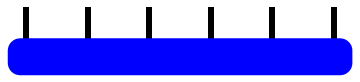
\includegraphics[width=0.4\linewidth]{include/p1}
\par\end{centering}
\end{figure}
\noindent 而矩阵乘积态,就是将这样的张量拆成更小的单元:
\begin{figure}[H]
\begin{centering}
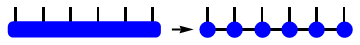
\includegraphics[width=0.6\linewidth]{include/p2}
\par\end{centering}
\end{figure}

\section*{矩阵乘积态的等价性}
\noindent 我们现在来证明任意有限维的$N$阶张量可以表示为带指标的N个矩阵的乘积:
\begin{equation}
	C_{i_{1},\cdots,i_{N}}=M_{i_{1}}^{\left[1\right]}M_{i_{2}}^{\left[2\right]}\cdots M_{i_{N}}^{\left[N\right]} .
\end{equation}
这种表示本质上是张量的分解,我们将$N$阶张量的指标组合,变为一矩阵:
\begin{equation}
	C_{i_{1},i_{2},\cdots,i_{N}}\rightarrow C_{i_{1},\left(i_{2},\cdots,i_{N}\right)}\rightarrow C_{m,n},
\end{equation}
括号表示张量指标合并,具体可以写为: $m=i_{1},\ n=i_{2}d^{N-2}+i_{3}d^{N-3}+\cdots+i_{N}d^{0}$. 我们接下来对矩阵 $C_{mn}$ 做奇异值分解:
\begin{equation}
	C_{m,n}=\sum_{\lambda=1}^{k}U_{m,\lambda}S_{\lambda}V_{\lambda,n}^{\dagger} .
\end{equation}
我们用左边的矩阵 $U$ 作为矩阵乘积的第一项:
\begin{equation}
	\left(M_{i_{1}}^{\left[1\right]}\right)_{1,a}=U_{i_{1},a} ,
\end{equation}
$M_{i_{1}}^{\left[1\right]}$ 是一个 $1\times k$ 矩阵。我们将剩余部分合并为新矩阵:
\begin{equation}
	\sum_{\lambda=1}^{k}S_{\lambda}V_{\lambda,n}^{\dagger}=D_{\lambda,i_{2},\cdots,i_{N}}\rightarrow D_{\left(\lambda,i_{2}\right),\left(i_{3},\cdots,i_{N}\right)}\rightarrow D_{m,n} ,
\end{equation}
其中 $m=\lambda k+i_{2},\ n=i_{3}d^{N-3}+\cdots+i_{N}d^{0}$. 继续做奇异值分解:
\begin{equation}
	D_{m,n}=\sum_{\lambda=1}^{k'}U_{m,\lambda}S_{\lambda}V_{\lambda,n}^{\dagger}.
\end{equation}
左边的矩阵 $U$ 作为第二项:
\begin{equation}
	\left(M_{i_{2}}^{\left[2\right]}\right)_{a,b}=U_{a,i_{2},b}.
\end{equation}
$M_{i_{2}}^{\left[2\right]}$ 是一个 $k\times k'$ 矩阵。重复以上操作,直到我们分解到最后一个指标 $i_{N}$ ,即 $D_{m,i_{N}}$,此时我们将 $\sum_{\lambda=1}^{k''}S_{\lambda}V_{\lambda,i_{N}}^{\dagger}$ 作为最后一个矩阵 $M_{i_{N}}^{\left[N\right]}$, 是一个 $k'' \times 1$ 矩阵。
经过一系列指标重组,奇异值分解后,我们将原来的$N$指标张量表示为了矩阵乘积态:
\begin{equation}
	C_{i_{1},\cdots,i_{N}}=M_{i_{1}}^{\left[1\right]}M_{i_{2}}^{\left[2\right]}\cdots M_{i_{N}}^{\left[N\right]}.
\end{equation}
我们可以用图形语言十分清楚地表示出以上过程:
\begin{figure}[H]
\begin{centering}
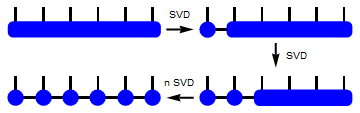
\includegraphics[width=0.6\linewidth]{include/p3}
\par\end{centering}
\end{figure}

\section*{表示的优势:矩阵压缩}
矩阵乘积态的形式有直接的物理意义。整个系统的多体态被表示为乐高积木一样由基本单元拼接而成,每个单元是一个三阶张量:
\begin{figure}[H]
\begin{centering}
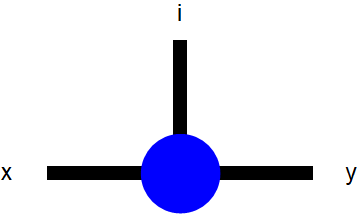
\includegraphics[width=0.3\linewidth]{include/p4}
\par\end{centering}
\end{figure}
\noindent 其中$i$指标是格点量子态,$x,y$可以看作其与左右系统之间的量子纠缠。这时这种表示的优越性就体现了出来,类似之前证明中的构造过程,我们可以将多体系统表示写为施密特分解的形式:
\begin{equation}
	\left|\psi\right\rangle =\sum_{\lambda}S_{\lambda}\left|\lambda\right\rangle _{A}\left|\lambda\right\rangle _{B}.
\end{equation}
其中 $\left|\lambda\right\rangle _{A},\left|\lambda\right\rangle _{B}$ 分别为$A,B$子系统的一组正交基。图形语言表示为:
\begin{figure}[H]
\begin{centering}
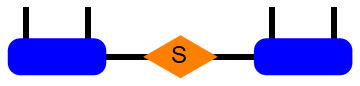
\includegraphics[width=0.4\linewidth]{include/p5}
\par\end{centering}
\end{figure}
\noindent 其中 $\left\{ S_{\lambda}\right\}$ 代表奇异值。奇异值可以用来做矩阵压缩,如果系统两部分之间纠缠不强,奇异值的谱往往衰减很快,我们只需保留为数不多的奇异值,就可以保留矩阵大部分的信息。

这样,我们可以在乘积态的每个相连的脚上做奇异值分解并保留有限个奇异值。经过这样的压缩操作后每个单元上 $x,y$ 指标维数都可以被控制在一个不大的上限内。

因此对于一个纠缠不强的多体态,我们可以用一系列维数不大的矩阵很好地近似表示出它。假设我们规定每组施密特分解保留不超过 $D$ 个奇异值,最终我们只需要 $NdD^{2}$ 个实数就能近似表示出这个多体态。这种表示对于格点数有线性的空间复杂度,效率远远高于原张量积表示指数增长的空间复杂度。这让我们可以研究格点较大的体系。

\section*{矩阵乘积态有效性}
\noindent 一个自然的问题是为什么MPS可以如此高效地表示多体态。事实上,张量积表示本身并没有任何冗余信息,对于一个任意的多体态,其所包含的信息随格点数增长就是指数的。因此MPS并不能高效的表示出任意的多体态,而仅仅对于希尔伯特空间内极少部分的态有效。幸运的是,我们真正关心的态往往都能用MPS表示出来。

首先,真实系统相互作用往往是局域的,这种局域相互作用表现在关联函数的指数衰减。同时,对于由局域的相互作用组成的哈密顿量,有两个重要的结论:
\begin{enumerate}
	\item 基态及低激发态纠缠熵满足面积律,对一维系统,表现为中间各处二分系统纠缠熵基本相同;
	\item 从直积态演化后在较长时间($N$的多项式数量级)内满足面积率。
\end{enumerate}
对此有一篇综述(\href{https://arxiv.org/abs/0808.3773}{Area laws for the entanglement entropy})详细讨论了局域哈密顿量下基态的纠缠性质。
\begin{figure}[H]
\begin{centering}
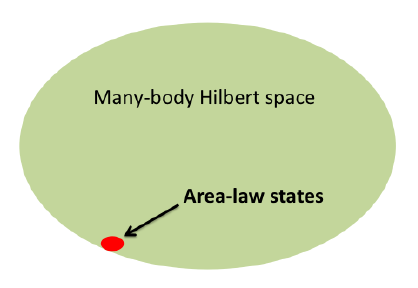
\includegraphics[width=0.5\linewidth]{include/p6}
\caption{满足面积律的态只占多体希尔伯特空间的极小一部分,然而这部分态恰恰是我们最关心的态。}
\par\end{centering}
\end{figure}
\noindent 对一维系统来说,纠缠熵面积律意味着系统纠缠熵不会随体系增大而增大,这样我们的表示矩阵的维数也可以被限制在一个可控的上限内。因此 MPS 态可以很好地表示局域算符组成的哈密顿量的基态,以及从直积态开始不太长时间内的含时演化。

\section*{矩阵乘积态物理量的表示}
\noindent 我们沿用上述张量表示规则,大部分物理量的计算变为一个张量网络的缩并。用图形语言可以清晰地表示出来。

\subsubsection*{内积:} 
\begin{figure}[H]
\begin{centering}
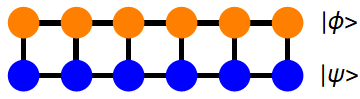
\includegraphics[width=0.45\linewidth]{include/p7}
\par\end{centering}
\end{figure}

\subsubsection*{局域算符期望值:} 
\begin{figure}[H]
\begin{centering}
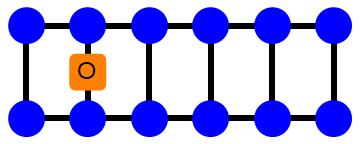
\includegraphics[width=0.4\linewidth]{include/p8}
\par\end{centering}
\end{figure}

\subsubsection*{关联函数:} 
\begin{figure}[H]
\begin{centering}
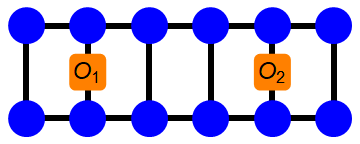
\includegraphics[width=0.4\linewidth]{include/p9}
\par\end{centering}
\end{figure}

\subsubsection*{纠缠熵:} 
\begin{figure}[H]
\begin{centering}
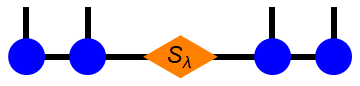
\includegraphics[width=0.4\linewidth]{include/p10}
\par\end{centering}
\end{figure}
\noindent 其中
\begin{equation}
	S=-\sum_{\lambda}S_{\lambda}\log\left(S_{\lambda}\right).
\end{equation}

\section*{矩阵乘积算符(MPO)}
对于一个多体算符,像态一样,我们可以将多体算符统一写为:
\begin{equation}
	O=\sum_{i_{1},\cdots,i_{N},i_{1}',\cdots,i_{N}'=1}^{d}C_{i_{1},\cdots,i_{N}}^{i_{1}',\cdots,i_{N}'}\left|i_{1}',\cdots,i_{N}'\right\rangle \left\langle i_{1},\cdots,i_{N}\right|.
\end{equation}
图形表示为:
\begin{figure}[H]
\begin{centering}
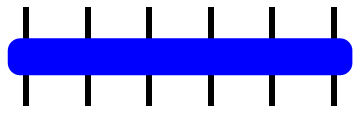
\includegraphics[width=0.4\linewidth]{include/p11}
\par\end{centering}
\end{figure}
\noindent 和态不同的是,局域算符组成的哈密顿量自然地可以写为矩阵乘积形式:
\begin{equation}
	O=\sum_{i_{1},\cdots,i_{N},i_{1}',\cdots,i_{N}'=1}^{d}M_{i_{1}',i_{1}}^{\left[1\right]}M_{i_{2}',i_{2}}^{\left[2\right]}\cdots M_{i_{N}',i_{N}}^{\left[N\right]}\left|i_{1}',\cdots,i_{N}'\right\rangle \left\langle i_{1},\cdots,i_{N}\right|.
\end{equation}
\begin{figure}[H]
\begin{centering}
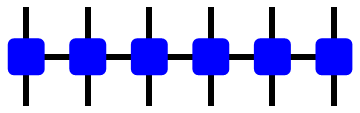
\includegraphics[width=0.4\linewidth]{include/p12}
\par\end{centering}
\end{figure}
\noindent MPO作用与MPS态后任然保持MPS结构:
\begin{figure}[H]
\begin{centering}
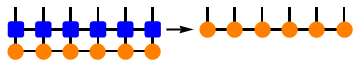
\includegraphics[width=0.6\linewidth]{include/p13}
\par\end{centering}
\end{figure}
\noindent 到这一步,我们将多体问题中会遇到的几乎所有问题表示为了矩阵乘积的形式。下面我们来考虑如何在这样的表示下求两个最基本的多体问题——求本征态和求态的含时演化。

\section*{求解本征态:DMRG算法基本思想}
\noindent 本征值问题本质上是对一个变分极小值问题:
\begin{equation}
	E\left[\psi\right]=\left\langle \psi\right|H\left|\psi\right\rangle.
\end{equation}
用图形语言表述:
\begin{figure}[H]
\begin{centering}
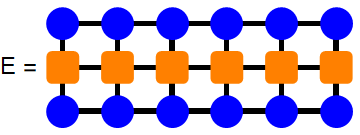
\includegraphics[width=0.4\linewidth]{include/p14}
\par\end{centering}
\end{figure}
\noindent 对于这种变分问题,我们可以采用局部优化的思路,在保持其他格点张量不变的情况下,对其中一个格点张量取变分极小值,再不断对不同格点做相同操作,最终这个矩阵乘积态会收敛到基态。

我们同样可以用简单的图形语言描述格点张量最优化的过程:
\begin{figure}[H]
\begin{centering}
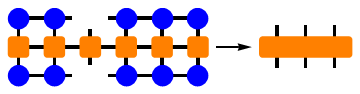
\includegraphics[width=0.6\linewidth]{include/p15}
\par\end{centering}
\end{figure}
\noindent 对于一个选定的格点,我们将原先的网络中除去这个格点张量的剩余部分做缩并操作,结果为一个6腿算符,将指标组合后对求矩阵的最小本征解就是局部最优解。

\section*{含时演化:TEBD算法基本思想}
态的演化可以看成是一个时间演化算符在态上的作用:
\begin{equation}
	\left|\psi\left(t\right)\right\rangle =e^{-iHt}\left|\psi\left(0\right)\right\rangle.
\end{equation}
TEBD 的核心思想是将由局域哈密顿量组成的算符拆成一系列短程作用的叠加。我们这里讨论只含近邻格点作用的哈密顿量,这样的哈密顿量可以写为:
\begin{equation}
	H=\sum_{i}H_{i,i+1}=\sum_{i=even}H_{i,i+i}+\sum_{i=odd}H_{i,i+1}.
\end{equation}
我们这样可以将哈密顿量分为两组,其中同一组内算符互相对易:
\begin{equation}
	\left[H_{i,i+1},H_{j,j+1}\right]=0,\ i=j\ \left(mod\ 2\right).
\end{equation}
我们要做的近似是,当 $\tau=t/n$  较小时,忽略奇偶成分之间非对易的成分:
\begin{equation}
	e^{-iH\tau}\approx\left(\prod_{i=even}e^{-i\tau H_{i,i+1}}\right)\cdot\left(\prod_{i=odd}e^{-i\tau H_{i,i+1}}\right).
\end{equation}
这样,我们可以将 $t$ 分割成 $n$ 份,并交替地作用奇偶算符。用图像语言表述为:
\begin{figure}[H]
\begin{centering}
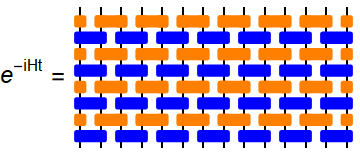
\includegraphics[width=0.5\linewidth]{include/p16}
\par\end{centering}
\end{figure}
\noindent 这种表示带来的一个问题是,这种网络作用在矩阵乘积态上会破坏矩阵乘积的结构。因此我们需要将作用算符表示成矩阵乘积算符的格式。方法也十分直接,我们直接用图形语言表示这个过程:
\begin{figure}[H]
\begin{centering}
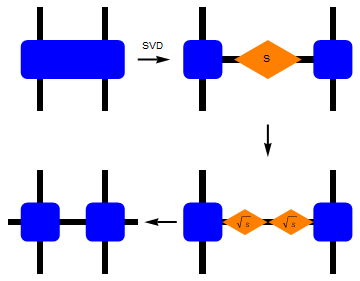
\includegraphics[width=0.4\linewidth]{include/p17}
\par\end{centering}
\end{figure}
\noindent 这样,以上每层操作都能用矩阵乘积算符表示出来。我们就可以不断地作用这样的 MPO 演化算符,并在过程中压缩 MPS 态矩阵,就实现了高效的时间多体态的含时演化。


\end{document}
